% Options for packages loaded elsewhere
\PassOptionsToPackage{unicode}{hyperref}
\PassOptionsToPackage{hyphens}{url}
\PassOptionsToPackage{dvipsnames,svgnames,x11names}{xcolor}
\documentclass[
  10pt,
  fontset=fandol]{ctexart}
\usepackage{xcolor}
\usepackage[margin=16mm]{geometry}
\usepackage{amsmath,amssymb}
\setcounter{secnumdepth}{-\maxdimen} % remove section numbering
\usepackage{iftex}
\ifPDFTeX
  \usepackage[T1]{fontenc}
  \usepackage[utf8]{inputenc}
  \usepackage{textcomp} % provide euro and other symbols
\else % if luatex or xetex
  \usepackage{unicode-math} % this also loads fontspec
  \defaultfontfeatures{Scale=MatchLowercase}
  \defaultfontfeatures[\rmfamily]{Ligatures=TeX,Scale=1}
\fi
\usepackage{lmodern}
\ifPDFTeX\else
  % xetex/luatex font selection
\fi
% Use upquote if available, for straight quotes in verbatim environments
\IfFileExists{upquote.sty}{\usepackage{upquote}}{}
\IfFileExists{microtype.sty}{% use microtype if available
  \usepackage[]{microtype}
  \UseMicrotypeSet[protrusion]{basicmath} % disable protrusion for tt fonts
}{}
\makeatletter
\@ifundefined{KOMAClassName}{% if non-KOMA class
  \IfFileExists{parskip.sty}{%
    \usepackage{parskip}
  }{% else
    \setlength{\parindent}{0pt}
    \setlength{\parskip}{6pt plus 2pt minus 1pt}}
}{% if KOMA class
  \KOMAoptions{parskip=half}}
\makeatother
\usepackage{longtable,booktabs,array}
\newcounter{none} % for unnumbered tables
\usepackage{calc} % for calculating minipage widths
% Correct order of tables after \paragraph or \subparagraph
\usepackage{etoolbox}
\makeatletter
\patchcmd\longtable{\par}{\if@noskipsec\mbox{}\fi\par}{}{}
\makeatother
% Allow footnotes in longtable head/foot
\IfFileExists{footnotehyper.sty}{\usepackage{footnotehyper}}{\usepackage{footnote}}
\makesavenoteenv{longtable}
\usepackage{graphicx}
\makeatletter
\newsavebox\pandoc@box
\newcommand*\pandocbounded[1]{% scales image to fit in text height/width
  \sbox\pandoc@box{#1}%
  \Gscale@div\@tempa{\textheight}{\dimexpr\ht\pandoc@box+\dp\pandoc@box\relax}%
  \Gscale@div\@tempb{\linewidth}{\wd\pandoc@box}%
  \ifdim\@tempb\p@<\@tempa\p@\let\@tempa\@tempb\fi% select the smaller of both
  \ifdim\@tempa\p@<\p@\scalebox{\@tempa}{\usebox\pandoc@box}%
  \else\usebox{\pandoc@box}%
  \fi%
}
% Set default figure placement to htbp
\def\fps@figure{htbp}
\makeatother
\setlength{\emergencystretch}{3em} % prevent overfull lines
\providecommand{\tightlist}{%
  \setlength{\itemsep}{0pt}\setlength{\parskip}{0pt}}
\usepackage{amsmath,amssymb,mathtools,needspace}
\xeCJKDeclareCharClass{CJK}{"2032,"0400->"04FF,"2160->"216B,"2460->"2473,"25A0,"25C7,"25CB,"25CF}
\IfFontExistsTF{Arial Unicode MS}{\xeCJKsetup{AutoFallBack=true}\setCJKfallbackfamilyfont{\CJKrmdefault}{Arial Unicode MS}}{}
\setcounter{secnumdepth}{0}
\setlength{\emergencystretch}{2em}
\allowdisplaybreaks
\usepackage{bookmark}
\IfFileExists{xurl.sty}{\usepackage{xurl}}{} % add URL line breaks if available
\urlstyle{same}
\hypersetup{
  pdftitle={边值问题的数值解法},
  colorlinks=true,
  linkcolor={Maroon},
  filecolor={Maroon},
  citecolor={Blue},
  urlcolor={Blue},
  pdfcreator={LaTeX via pandoc}}

\title{边值问题的数值解法}
\author{}
\date{}

\begin{document}
\maketitle

\subsection{5.7 边值问题的数值解法}\label{ux8fb9ux503cux95eeux9898ux7684ux6570ux503cux89e3ux6cd5}

在具体求解微分方程时，必须附加某种定解条件。微分方程和定解条件一起组成定

\href{../../source-images/pdf-148.jpeg}{原页}

（接上页）解问题。对于高阶微分方程，定解条件通常有两种给法：一种是给出了积分曲线在初始时刻的性态，这类条件称为\textbf{初始条件}，相应的定解问题称为\textbf{初值问题}；另一种是给出了积分曲线首末两端的性态，这类条件则称为\textbf{边界条件}，相应的定解问题称为\textbf{边值问题}。

以二阶方程

\[
y''=f(x,y,y')
\tag{5.7.1}
\]

为例，其初始条件的给法是

\[
y(a)=\alpha,\quad y'(a)=m.
\tag{5.7.2}
\]

前面已经研究过这种初值问题的数值解法。

设在区间 \(a<x<b\) 上求解方程（5.7.1），则边界条件可以给为

\[
y(a)=\alpha,\quad y(b)=\beta.
\tag{5.7.3}
\]

\subsubsection{5.7.1 试射法}\label{ux8bd5ux5c04ux6cd5}

可以用所谓``试射法''来求解边值问题（5.7.1）、（5.7.3）。这种方法的基本思想是设法将边值问题转化为初值问题来求解，即依据边界条件（5.7.3）寻求与它等价的初始条件（5.7.2），也就是说，反复调整初始时刻的斜率值 \(y'(a)=m\)，使初值问题（5.7.1）、（5.7.2）的积分曲线 \(y=y(x)\) 能``命中''\(y(b)=\beta\)（见图 5.5）。

试射法的计算过程很简单。设凭经验能够提供 \(m\) 的两个预测值 \(m_1,m_2\)，分别按这两个斜率值``试射''------求解相应的初值问题（5.7.1）、（5.7.2），从而获得 \(y(b)\) 的两个结果 \(\beta_1,\beta_2\)。如果 \(\beta_1\) 与 \(\beta_2\) 均不满足预定的精度，就用线性插值方法校正 \(m_1,m_2\) 得新的斜率值

\[
m_3=m_1+\frac{m_2-m_1}{\beta_2-\beta_1}(\beta-\beta_1),
\]

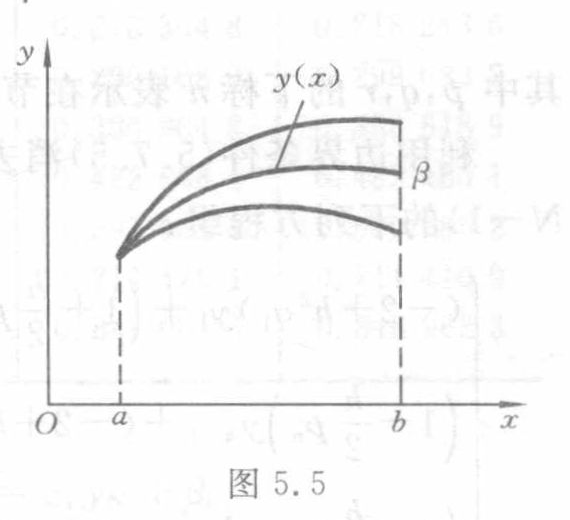
\includegraphics[width=0.85\linewidth,height=\textheight,keepaspectratio,alt={图 5.5（原图）试射法示意}]{../assets/ch05b/figure-5-5.png}

图 5.5（原图）符号与图意：坐标轴 \(x,y\)，原点 \(O\)，横轴端点 \(a,b\)，目标右端值 \(\beta\)，积分曲线标记 \(y(x)\)。三条曲线从 \(x=a\) 的同一左端点出发，在 \(x=b\) 处到达不同高度；\(y(x)\) 指向达到目标 \(\beta\) 的中间曲线。端点位置以竖虚线标出；图中未给出具体函数或数值。

然后再按斜率值 \(m_3\) 试射，求解相应的初值问题（5.7.1）、（5.7.2），又得新的结果 \(y(b)=\beta_3\)。继续这一过程，直到计算结果 \(y(b)\) 与 \(\beta\) 相当符合为止。

上述试射法过分依赖于经验，局限性大。下面介绍求解边值问题的差分方法。

\subsubsection{5.7.2 差分方程的建立}\label{ux5deeux5206ux65b9ux7a0bux7684ux5efaux7acb}

应用差分方法的关键，在于恰当地选取差商逼近微分方程中的导数。我们知道，逼近一阶导数 \(y'(x)\) 可用向前差商 \(\dfrac{y(x+h)-y(x)}h\)，亦可用向后差商 \(\dfrac{y(x)-y(x-h)}h\) 或中心差商 \(\dfrac{y(x+h)-y(x-h)}{2h}\)。中心差商是向前差商与向后差商的算术平均。为逼近二阶导数 \(y''(x)\)，一般用二阶差商------向前差商的向后差商（即向后差商的向前差商）

\href{../../source-images/pdf-149.jpeg}{原页}

\[
y''(x)\approx\frac{\dfrac{y(x+h)-y(x)}h-\dfrac{y(x)-y(x-h)}h}{h}
=\frac{y(x+h)-2y(x)+y(x-h)}{h^2}.
\]

设将积分区间 \([a,b]\) 划分为 \(N\) 等份，步长 \(h=\dfrac{b-a}{N}\)，节点 \(x_n=x_0+nh,n=0,1,\cdots,N\)。用差商替代相应的导数，可将边值问题（5.7.1）、（5.7.3）离散化得下列计算公式：

\[
\frac{y_{n+1}-2y_n+y_{n-1}}{h^2}=f\left(x_n,y_n,\frac{y_{n+1}-y_{n-1}}{2h}\right)\qquad(n=1,2,\cdots,N-1),
\tag{5.7.4}
\]

\[
y_0=\alpha,\quad y_N=\beta.
\tag{5.7.5}
\]

如果函数 \(f\) 是非线性的，那么所归结出的差分方程也是非线性的，这时实际求解比较困难。

如果所给方程（5.7.1）是如下形式的线性方程：

\[
y''+p(x)y'+q(x)y=r(x),
\tag{5.7.6}
\]

则差分方程（5.7.4）相应的形式为

\[
\frac{y_{n+1}-2y_n+y_{n-1}}{h^2}+p_n\frac{y_{n+1}-y_{n-1}}{2h}+q_ny_n=r_n\qquad(n=1,\cdots,N-1),
\tag{5.7.7}
\]

其中 \(p,q,r\) 的下标 \(n\) 表示在节点 \(x_n\) 取值。

利用边界条件（5.7.5）消去式（5.7.7）中的 \(y_0\) 和 \(y_N\)，整理得到关于 \(y_n\)（\(1\le n\le N-1\)）的下列方程组：

\[
\begin{cases}
\displaystyle(-2+h^2q_1)y_1+\left(1+\frac h2p_1\right)y_2=h^2r_1-\left(1-\frac h2p_1\right)\alpha,\\[6pt]
\displaystyle\left(1-\frac h2p_n\right)y_{n-1}+(-2+h^2q_n)y_n+\left(1+\frac h2p_n\right)y_{n+1}=h^2r_n\quad(2\le n\le N-2),\\[6pt]
\displaystyle\left(1-\frac h2p_{N-1}\right)y_{N-2}+(-2+h^2q_{N-1})y_{N-1}=h^2r_{N-1}-\left(1+\frac h2p_{N-1}\right)\beta.
\end{cases}
\tag{5.7.8}
\]

这样归结出的方程组是所谓\textbf{三对角型}的，即

\[
\begin{pmatrix}
-2+h^2q_1 & 1+\dfrac h2p_1 & & & \\
1-\dfrac h2p_2 & -2+h^2q_2 & 1+\dfrac h2p_2 & & \\
& \ddots & \ddots & \ddots & \\
& & 1-\dfrac h2p_{N-2} & -2+h^2q_{N-2} & 1+\dfrac h2p_{N-2} \\
& & & 1-\dfrac h2p_{N-1} & -2+h^2q_{N-1}
\end{pmatrix},
\]

\href{../../source-images/pdf-150.jpeg}{原页}

因为它的系数矩阵仅在主对角线及其相邻的两条对角线上有非零元素。求解这种三对角型方程组，用所谓\textbf{追赶法}特别有效。在 7.4.3 节将介绍追赶法。

\textbf{例 5.7} 用差分方法解边值问题 \(\begin{cases}y''-y=x,\quad0<x<1,\\y(0)=0,\quad y(1)=1.\end{cases}\)

\textbf{解} 取步长 \(h=0.1\)，节点 \(x_n=\dfrac n{10}\)（\(n=0,1,2,\cdots,10\)），差分方程（5.7.8）的形式是

\[
\begin{pmatrix}
-2-10^{-2}&1&&&\\
1&-2-10^{-2}&1&&\\
&\ddots&\ddots&\ddots&\\
&&1&-2-10^{-2}&1\\
&&&1&-2-10^{-2}
\end{pmatrix}
\begin{pmatrix}y_1\\y_2\\\vdots\\y_8\\y_9\end{pmatrix}
=
\begin{pmatrix}0.1\times10^{-2}\\0.2\times10^{-2}\\\vdots\\0.8\times10^{-2}\\-1+0.9\times10^{-2}\end{pmatrix}.
\]

表 5.11 列出了差分方法的计算结果，表中最末一列是按解的表达式

\[
y=\frac{2(\mathrm e^x-\mathrm e^{-x})}{\mathrm e-\mathrm e^{-1}}-x
\]

算出的准确值。

\textbf{表 5.11}

{\def\LTcaptype{none} % do not increment counter
\begin{longtable}[]{@{}lrr@{}}
\toprule\noalign{}
\(x_n\) & \(y_n\) & \(y(x_n)\) \\
\midrule\noalign{}
\endhead
\bottomrule\noalign{}
\endlastfoot
0.1 & 0.0704894 & 0.0704673 \\
0.2 & 0.1426836 & 0.1426409 \\
0.3 & 0.2183048 & 0.2182436 \\
0.4 & 0.2991089 & 0.2990332 \\
0.5 & 0.3869042 & 0.3868189 \\
0.6 & 0.4835684 & 0.4834801 \\
0.7 & 0.5910684 & 0.5909852 \\
0.8 & 0.7114791 & 0.7114109 \\
0.9 & 0.8470045 & 0.8469633 \\
\end{longtable}
}

附带指出，在应用上，有时边界条件按以下方式给出：

当 \(x=a\) 时，\(y'=\alpha_0y+\beta_0\)；当 \(x=b\) 时，\(y'=\alpha_1y+\beta_1\)。

这里 \(\alpha_0,\beta_0,\alpha_1,\beta_1\) 均为已知常数，这时，边界条件中所包含的微商也要替换成相应的差商

\[
\frac{y_1-y_0}{h}=\alpha_0y_0+\beta_0,\qquad
\frac{y_N-y_{N-1}}h=\alpha_1y_N+\beta_1.
\]

它们和差分方程（5.7.7）一起，仍然构成包含 \(N+1\) 个未知数的线性方程组。

\subsubsection{5.7.3 差分问题的可解性}\label{ux5deeux5206ux95eeux9898ux7684ux53efux89e3ux6027}

我们知道，通过自变量的适当变换可以消除线性方程（5.7.6）中的一阶导数项。下面仅就缺一阶导数项的方程来讨论这一问题。考察边值问题

\[
\begin{cases}
y''-q(x)y=r(x),\\
y(a)=\alpha,\quad y(b)=\beta.
\end{cases}
\tag{5.7.9}
\]

这里假定 \(q(x)\ge0\)，其对应的差分问题是

\[
\begin{cases}
\displaystyle\frac{y_{n+1}-2y_n+y_{n-1}}{h^2}-q_ny_n=r_n\quad(n=1,2,\cdots,N-1),\\[6pt]
y_0=\alpha,\quad y_N=\beta.
\end{cases}
\tag{5.7.10}
\]

\href{../../source-images/pdf-151.jpeg}{原页}

现在论证差分问题的可解性。由于式（5.7.10）是关于变量 \(y_n\)（\(n=0,1,2,\cdots,N\)）的线性方程组，要证明它的解存在唯一，只要证明对应的齐次方程组只有零解。为此，我们引进下述极值原理。

\textbf{定理 5.2} 对于一组不全相等的数 \(y_n\)（\(n=0,1,\cdots,N\)），记

\[
l(y_n)=\frac{y_{n+1}-2y_n+y_{n-1}}{h^2}-q_ny_n,\quad q_n\ge0\qquad(n=1,2,\cdots,N-1).
\]

假定 \(l(y_n)\ge0\)（\(n=1,2,\cdots,N-1\)），则 \(y_n\) 的正的最大值只能是 \(y_0\) 或 \(y_N\)；如果 \(l(y_n)<0\)（\(n=1,2,\cdots,N-1\)），则 \(y_n\) 的负的最小值只能是 \(y_0\) 或 \(y_N\)。

\textbf{证明} 用反证法。考察 \(l(y_n)\ge0\) 的情形，设 \(y_m\)（\(0<m<N\)）是正的最大值，即 \(y_m=\max_{0\le n\le N}y_n=M>0\)，且 \(y_{m-1}\) 和 \(y_{m+1}\) 中至少有一个小于 \(M\)，此时有

\[
l(y_m)=\frac{y_{m+1}-2y_m+y_{m-1}}{h^2}-q_my_m<\frac{M-2M+M}{h^2}-q_mM=-q_mM,
\]

由于 \(q_m\ge0,M>0\)，故由上式推出 \(l(y_m)<0\)，此与题设矛盾。

此外，\(l(y_n)<0\) 的情形可类似地进行讨论。证毕。

作为这一定理的推论有如下定理。

\textbf{定理 5.3} 差分问题式（5.7.10）的解存在并且是唯一的。

\textbf{证明} 只要证明对应的齐次方程组

\[
\begin{cases}
\displaystyle l(y_n)=\frac{y_{n+1}-2y_n+y_{n-1}}{h^2}-q_ny_n=0\quad(n=1,2,\cdots,N-1),\\[6pt]
y_0=y_N=0
\end{cases}
\]

只有零解。由于这里 \(l(y_n)=0\)（\(n=1,2,\cdots,N-1\)），由极值原理知，\(y_n\) 的正的最大值和负的最小值只能是 \(y_0\) 或 \(y_N\)，而按边界条件 \(y_0=y_N=0\)，故所有的 \(y_n\)（\(n=0,1,\cdots,N\)）全为零。证毕。

\subsubsection{5.7.4 差分方法的收敛性}\label{ux5deeux5206ux65b9ux6cd5ux7684ux6536ux655bux6027}

现在运用极值原理论证差分方法的收敛性并估计误差。

\textbf{定理 5.4} 设 \(y_n\) 是差分问题式（5.7.10）的解，而 \(y(x_n)\) 是边值问题（5.7.9）的解 \(y(x)\) 在节点 \(x_n\) 的值，则截断误差 \(e_n=y(x_n)-y_n\) 有下列估计式：

\[
|e_n|\le\frac{M(b-a)^2}{96}h^2,\qquad
M=\max_{a\le x\le b}|y^{(4)}(x)|.
\tag{5.7.11}
\]

\textbf{证明} 由 Taylor 展开，易得

\[
\begin{cases}
\displaystyle\frac{y(x_{n+1})-2y(x_n)+y(x_{n-1})}{h^2}-q_ny(x_n)=r_n+\frac{h^2}{12}y^{(4)}(\xi_n),\quad x_{n-1}<\xi_n<x_{n+1},\\[6pt]
y(x_0)=\alpha,\quad y(x_N)=\beta.
\end{cases}
\tag{5.7.12}
\]

\begin{quote}
校注（agent 补充）：定理 5.2 的负最小值一侧，原书确实写作严格条件 \(l(y_n)<0\)；定理 5.3 却在 \(l(y_n)=0\) 时同时引用正最大值、负最小值结论。此处原文均照录。补足该引用的方法是对 \(-y_n\) 应用定理 5.2 的 \(l\ge0\) 一侧（利用 \(l\) 的线性），从而排除负最小值；无需改动原书方程。
\end{quote}

\href{../../source-images/pdf-152.jpeg}{原页}

将式（5.7.12）与式（5.7.10）相减，知截断误差 \(e_n=y(x_n)-y_n\) 满足

\[
\begin{cases}
\displaystyle l(e_n)=\frac{e_{n+1}-2e_n+e_{n-1}}{h^2}-q_ne_n=\frac{h^2}{12}y^{(4)}(\xi_n),\\[6pt]
e_0=e_N=0,
\end{cases}
\]

其中 \(\xi_n\) 一般是不知道的。于是转向下列差分问题：

\[
\begin{cases}
\displaystyle l(\varepsilon_n)=\frac{\varepsilon_{n+1}-2\varepsilon_n+\varepsilon_{n-1}}{h^2}-q_n\varepsilon_n=-\frac{h^2}{12}M,\\[6pt]
\varepsilon_0=\varepsilon_N=0,
\end{cases}
\tag{5.7.13}
\]

其中 \(M=\max_{a\le x\le b}|y^{(4)}(x)|\)。首先证明上述两个差分问题的解存在下列关系：

\[
|e_n|\le\varepsilon_n\qquad(n=0,1,\cdots,N).
\tag{5.7.14}
\]

事实上，由于

\[
l(\varepsilon_n)=-\frac{h^2}{12}M\le-\frac{h^2}{12}|y^{(4)}(\xi_n)|=-|l(e_n)|,
\]

故有

\[
l(\varepsilon_n-e_n)\le0,\qquad l(\varepsilon_n+e_n)\le0.
\]

又

\[
\varepsilon_0-e_0=\varepsilon_N-e_N=0,\qquad\varepsilon_0+e_0=\varepsilon_N+e_N=0,
\]

利用定理 5.2，知 \(\varepsilon_n-e_n\ge0,\varepsilon_n+e_n\ge0\)，即式（5.7.14）成立。

差分问题（5.7.13）的解仍不易直接求得，于是进一步考察

\[
\begin{cases}
\displaystyle\tilde l(\rho_n)=\frac{\rho_{n+1}-2\rho_n+\rho_{n-1}}{h^2}=-\frac{h^2}{12}M,\\[6pt]
\rho_0=\rho_N=0.
\end{cases}
\tag{5.7.15}
\]

这里 \(\tilde l(\rho_n-\varepsilon_n)=-q_n\varepsilon_n\le0\)，又 \(\rho_0-\varepsilon_0=\rho_N-\varepsilon_N=0\)，故由定理 5.2（注意，当 \(q_n=0\) 时，\(l(\tilde y_n)\) 就是 \(l(y_n)\)）知 \(\rho_n-\varepsilon_n\ge0\)，即 \(\varepsilon_n\le\rho_n\)，于是有 \(|e_n|\le\varepsilon_n\le\rho_n\)。

然而 \(\rho_n\) 是容易求出的。求解差分问题（5.7.15）所对应的边值问题

\[
\begin{cases}
\displaystyle\rho''=-\frac{h^2}{12}M,\\[6pt]
\rho(a)=\rho(b)=0,
\end{cases}
\]

解得

\[
\rho(x)=\frac{h^2}{24}M(x-a)(b-x).
\]

容易验证 \(\rho_n=\rho(x_n)\) 是差分问题（5.7.15）的解，注意到 \(\rho(x)\) 在点 \(x=\dfrac{a+b}2\) 达到最大值

\[
\rho\left(\frac{a+b}2\right)=\frac{M(b-a)^2}{96}h^2,
\]

因此有估计式（5.7.11）。证毕。

据估计式（5.7.11）知，当 \(h\to0\) 时有 \(e_n\to0\)，这表明差分方法（5.7.10）是收敛的。

\begin{quote}
校注（agent 补充，ch05b-E006）：式（5.7.15）后括注的原图在 \(y\) 上方印波浪号，即 \(l(\tilde y_n)\)，这里照录。按该式定义与``当 \(q_n=0\) 时''的上下文，此处疑将波浪号排错位置，预期为 \(\tilde l(y_n)\)，即去掉零阶项后的算子；原文并未定义 \(\tilde y_n\)。
\end{quote}

\subsection{本节覆盖原页的校注记录}\label{ux672cux8282ux8986ux76d6ux539fux9875ux7684ux6821ux6ce8ux8bb0ux5f55}

下列记录按原页关联，含同页相邻小节的校注；计算时同时读取上文校注和完整原页。

\begin{itemize}
\tightlist
\item
  \texttt{ch05b-E006}：原书 PDF 页 152
\end{itemize}

\end{document}
